%!TEX TS-program = xelatex
% Much of the initial version of this lab manual was taken from Jonathan Peelle's lab manual.
% See original source here: https://github.com/jpeelle/peellelab_manual/

\documentclass[letterpaper,11pt,oneside]{memoir}

% ---------- Core packages ----------
\usepackage{xcolor}
\usepackage{xunicode,fontspec,xltxtra}
\usepackage{libertine}

\usepackage{graphicx}
\usepackage{booktabs}
\usepackage{array,ragged2e}
\usepackage{enumitem}
\usepackage{multicol}
\usepackage{xurl}
\usepackage{csquotes}
\usepackage{framed} % provides the shaded environment

% ---------- Hyperref (load late) ----------
\usepackage[pdftitle={Smith Lab Manual}, pdfauthor={David V. Smith}, colorlinks=true, urlcolor=blue]{hyperref}

% ---------- Formatting helpers ----------
\defaultfontfeatures{Ligatures=TeX}
\renewcommand{\UrlFont}{\ttfamily\footnotesize}

\definecolor{shadecolor}{gray}{0.9}

\setsecnumdepth{section}
\maxtocdepth{subsection}
\chapterstyle{article}

\newcommand{\pref}[1]{page~\pageref{#1}}
\newcommand{\Sref}[1]{Section~\ref{#1}}

\setlength{\droptitle}{1in}
\checkandfixthelayout % for memoir class

\begin{document}

\title{Smith Lab Manual\thanks{Code and version history: \url{https://github.com/DVSneuro/smithlab_manual}}}
\author{David V. Smith\\Department of Psychology and Neuroscience\\Temple University}
\date{\today}

\maketitle
\pagestyle{titlingpage}

\cleardoublepage
\frontmatter
\tableofcontents
\cleardoublepage

\mainmatter
\pagestyle{headings}

%%%%%%%%%%%%%%%%%%%%%
\chapter{Introduction}

The Smith Lab is a place for careful, collaborative science. We aim to better understand how the brain supports social and economic decision-making, and how these processes shape health and well-being across the lifespan. We also aim to prepare trainees to make lasting contributions through rigorous research, clear communication, and strong scientific habits (learning, reproducibility, and good teamwork).

This lab manual is your starting point for understanding how the lab works---what is expected, how we coordinate, and what norms help things run smoothly. You can find public information about the lab here:

\begin{itemize}[noitemsep]
\item Website: \url{https://sites.temple.edu/neuroeconlab/}
\item GitHub: \url{https://github.com/DVS-Lab}
\item Bluesky: \href{https://bsky.app/profile/did:plc:uql7gbrp52dxmxyfujst5yqp}{\texttt{@dvsmith.bsky.social}}
\end{itemize}

\noindent Lab members also use the following internal tools:

\begin{itemize}[noitemsep]
\item Slack: \url{https://smithlab-workspace.slack.com}
\item Slab: \url{https://smithlab.slab.com/}
\end{itemize}

This manual contains stable policies and lab-wide expectations. Day-to-day implementation (procedures, templates, step-by-step instructions) lives on Slab so it can be updated by anyone. Slack is our main platform for coordination and decisions. Use channels and threads for project-related work rather than DMs. Any information that is private, sensitive, or participant-identifying must be stored only in approved, secure locations. (For more on communication and shared tools, see \Sref{sec:communicationInLab} on \pref{sec:communicationInLab}.)

\begin{shaded}
\noindent Lab documentation---including this manual and Slab---is assumed to be accurate. If something is unclear, out of date, or missing, say so. You are encouraged to update Slab pages directly or raise issues at lab meeting. When you are unsure whether a policy or instruction still applies, ask. Do not rely on informal norms that contradict what is written down.
\end{shaded}

Finally, Temple policies always take precedence over lab policies. This includes policies related to accommodations, health and safety, reporting obligations, and university codes of conduct.


%%%%%%%%%%%%%%%%%%%%%
\chapter{About the Lab}

The lab runs on finite time and funding. We have to use both well. In practice, that means two things matter most: (a) solid scientific work that others can learn from (papers, methods, data, and code), and (b) trainees who leave here with strong skills and good judgment. Those goals rise and fall together.

\section{Our Values}

\subsection{Respect for Diversity}
As a first-generation college student from a low-income area of South Carolina, I recognize the importance of a lab culture where people from different backgrounds can thrive. Your feedback is welcome---about lab culture, materials, scheduling, or anything else. When lab activities conflict with religious observances or personal needs, let me know so we can make reasonable accommodations.

\subsection{Impactful Science}
Our goal is to do science that matters---within our fields and outside them. That means asking important questions, using valid methods, and communicating results clearly. As you work, think about how your work could be reused or extended by others.

\subsection{Skill Development}
Success in science depends on more than technical know-how. My goal is for everyone in the lab to develop a broad, transferable skillset---spanning methods, computation, writing, collaboration, and project management. Core areas include:

\begin{figure}[ht]
\centering
\includegraphics[width=\textwidth]{figures/skillrange.jpg}
\caption{A range of skills are needed to become an effective scientist in academia or industry.}
\end{figure}

\begin{itemize}[noitemsep]
\item \textbf{Methods \& Technology}: Know how your tools work, when they are appropriate, and what their limits are.
\item \textbf{Quantitative \& Computational}: Write and adapt code for analysis, and understand the statistical principles behind your work.
\item \textbf{Design \& Interpretation}: Ask good questions, design clean studies, and interpret results carefully in context.
\item \textbf{Management \& Leadership}: Track progress, manage timelines, and help mentor others as your experience grows.
\item \textbf{Communication \& Teamwork}: Communicate clearly in writing and speech, and work productively as part of a team.
\end{itemize}

\section{Funding and Stewardship}
Most of the lab’s work is supported by external grants, including awards from NIH. These grants fund personnel, equipment, participant payments, and infrastructure. Our current NIH-funded work runs through \textbf{2027}, and we are actively submitting proposals to continue our work on \textbf{aging and decision making}. Other proposals target connected areas, including \textbf{noninvasive brain stimulation} (building on prior R21/R03 work), the \textbf{ABCD Study}, and \textbf{social determinants of health}. A current summary of funded and pending projects is maintained in lab documentation (see Slab or OneDrive).

\paragraph{Effort, scope, and PI decision-making.}
NIH (and other sponsors) require that effort charged to a grant accurately reflects the work performed and aligns with the approved scope. Grant funds cannot be used to support unrelated activities.

For sponsored work, assigned tasks and deadlines are part of the role. As PI, I am responsible for sponsor compliance, project execution, and allocating effort where it best supports the aims. Final decisions about priorities, scope, and task assignments rest with me.

This is not about micromanaging. It is how funded research stays on track. When you anticipate a problem (skills, bandwidth, timeline), tell me early so we can adjust.

\section{How We Work}

\subsection{Training}
\label{sec:training}
We use an apprenticeship model: skills are passed along person-to-person, and everyone is expected to teach forward. When you learn a method, analysis, or procedure from someone else, document it clearly and update Slab so the next person can learn it faster. This is a core part of our lab culture and our ability to operate at scale.

You may also learn through collaborations beyond the lab. Treat those experiences as a chance to do careful work, learn something useful, and bring that value back to the group.

\subsection{Planning}
Everyone in the lab should have both short- and long-term goals and revisit them regularly. Plans, deadlines, and updates should be visible in Slack and/or Slab so collaborators can see what is happening. When a deadline slips or priorities change, say so early and write it down.

\subsection{Feedback}
You will receive feedback from me, other faculty, peers, reviewers, and collaborators. Some will be positive. Some will be critical. The point is improvement and progress.

I tend to focus quickly on next steps and troubleshooting. Ask directly when you need more clarity on what is going well (or what to prioritize). I give the most detailed feedback on fellowship applications, posters, talks, and manuscripts. Plan ahead; feedback is much more helpful when we are not up against a deadline.

For manuscripts, start with a paragraph-level outline (see \Sref{sec:ms_general} on \pref{sec:ms_general}) and reserve time to discuss. Do not send a full draft cold.


%%%%%%%%%%%%%%%%%%%%%
\chapter{Being in the Lab}

The lab functions as a team. We have different roles and responsibilities, all of which matter for our success. This chapter describes expectations that apply to everyone, plus role-specific expectations for common positions in the lab.

\begin{shaded}
\noindent Being in the lab generally means being physically present when possible. Some work can be done remotely (and sometimes remote work is necessary), but training, troubleshooting, and collaboration are often faster and easier in person.
\end{shaded}

\section{Everyone}

\subsection{Professionalism}
Professionalism in a research lab is mostly about being reliable, transparent, and easy to work with. In practice:

\begin{itemize}[noitemsep]
\item \textbf{Reliability}: Keep commitments. When a deadline will slip, communicate early and update the plan rather than going silent.
\item \textbf{Time management}: Manage your time so others are not waiting on you. When you are stuck, ask for help before you lose a lot of time spinning your wheels.
\item \textbf{Adaptability}: Research changes quickly. When plans change, adjust and move forward.
\item \textbf{Accountability}: Own mistakes, fix what you can, and document what changed.
\item \textbf{Honesty and integrity}: Be truthful about progress, contributions, and effort. Never do anything that jeopardizes data integrity or participant privacy. When you have concerns about research integrity, bring them to me promptly.
\end{itemize}

\subsection{Work visibility and documentation}
\label{sec:documentation}

We use shared systems so projects are easy to collaborate on, hand off, and reproduce. The goal is not to track every minute. The goal is to make sure that key decisions, current status, and next steps are visible to the people who need them.

\begin{itemize}[noitemsep]
\item Use Slack channels/threads for day-to-day updates, questions, and quick decisions.
\item After meetings, post a short summary (what we decided + who is doing what next).
\item Keep durable materials on Slab (project pages, procedures, templates, and “how-to” notes).
\end{itemize}

If someone else would need the information to continue your work (including you in six months), it should not live only in private notes or DMs.

\subsection{Research credit (independent study / collaborative research)}

Undergraduates and graduate students may participate in lab research for graded course credit (e.g., independent study / collaborative research). I assign grades using the NSCI Independent Study Evaluation form, which rates performance on a 1--5 scale across areas that matter for doing good research.

The evaluation covers (among other things): understanding of relevant science, study design/critical thinking, quality and care in data collection (when applicable), data management and organization, communication (responsiveness and clarity), preparation/participation in lab meetings (when relevant), time management, initiative, reliability in following through on commitments, and being a constructive member of the lab community.

\paragraph{Time expectation.}
Each 1 credit hour of research generally corresponds to \textbf{3--4 hours per week} of lab work during the term (unless explicitly arranged otherwise). This time should be scheduled, consistent, and visible to your supervisor.

\paragraph{No double counting of effort.}
Hours used to earn course credit must be \textbf{separate} from any paid lab employment or other sponsored effort. You may not count the same work hours toward both pay and research credit.

\paragraph{How you demonstrate progress.}
Because research credit is graded, you should be able to point to clear evidence of progress (e.g., recruitment logs, QC notes, analysis outputs, draft text, figures, documentation updates). Updates should be visible in the relevant Slack channels/threads, and durable procedures should be maintained on Slab.

\paragraph{What earns an A.}
An A reflects performance that is consistently strong and reliable. Typical features include: showing up prepared, completing assigned work carefully (with minimal avoidable errors), communicating early when something is blocked, taking initiative to solve problems or improve workflows, and leaving the project in a better state than you found it (cleaner documentation, better organization, small improvements that help others).

\paragraph{What leads to mediocre or failing grades (rare).}
Lower grades are uncommon, but when they happen they usually reflect not doing the work: repeated missed shifts or deadlines without communication, incomplete tasks that others must clean up, disappearing during the semester, or patterns of carelessness that persist after feedback. If something is not going to get done, the fix is almost always early, honest communication so we can adjust scope or reassign tasks.

\subsection{Shared space norms}
We share a relatively small space, so please be thoughtful of others and of participants.

\begin{itemize}[noitemsep]
\item With few exceptions, \textbf{do not come to the lab when you are sick}. Notify the lab manager (or me) and update the lab calendar when you will be out.
\item Keep the lab clean (especially common areas). Do not leave food, drinks, or trash in the lab.
\item Avoid strong perfumes/colognes (for coworkers and participants).
\item Minimize distractions: silence devices when possible; take personal calls outside the lab.
\end{itemize}

\section{The Principal Investigator}
As PI, I am responsible for the lab's scientific direction, funding strategy, mentoring, and sponsor compliance. You can generally expect me to:
\begin{itemize}[noitemsep]
\item Set the lab's scientific priorities over the next several years.
\item Obtain funding to support the science and the people doing it.
\item Meet regularly, provide feedback on scholarly work, and help remove barriers to progress.
\item Support professional development (letters, networking, and conference opportunities when feasible).
\end{itemize}

Working with me tends to go best when you double-check your work, keep projects moving without repeated reminders, and document what you learn so the next person can benefit (see \Sref{sec:training} on \pref{sec:training}).

\section{Post-baccalaureate Researchers}
We are fortunate to employ full-time post-baccalaureate researchers (post-baccs) who function as research coordinators and/or lab managers. They help run day-to-day operations and may also lead projects and mentor more junior lab members. I expect post-baccs to excel in reliability, communication, and follow-through. They may assign tasks and coordinate timelines on my behalf.

\begin{shaded}
\noindent Post-bacc coordinators may communicate lab procedures, priorities, and assignments that reflect lab leadership decisions. When you have concerns about a request, raise them with me promptly, but do not ignore or delay task execution while concerns sit unresolved.
\end{shaded}

\section{Post-doctoral Researchers}
Postdoctoral researchers bring expertise from prior training and are here to develop an increasingly independent program of research. I expect postdocs to take ownership of projects, contribute to grant writing and scholarly products, and help mentor others when appropriate. Postdoc salaries generally follow NIH guidelines (regardless of the source of funding).

\section{PhD Students}
PhD students are expected to develop deep expertise in their topic area and make steady progress toward publishable work. In general, I expect PhD students to:
\begin{itemize}[noitemsep]
\item Stay current with the literature relevant to their projects (see \Sref{sec:literature} on \pref{sec:literature}).
\item Make steady progress on data, analysis, and writing.
\item Seek training opportunities, fellowships, and awards when appropriate.
\item Build core competencies in analysis, coding, and scientific writing (see \Sref{sec:coding} on \pref{sec:coding}).
\end{itemize}

\paragraph{A note on PhD student funding.}
Most PhD students are supported through a mix of TA and RA appointments across the academic year (typically nine months), and some students teach many semesters across the program, including summers. We have been fortunate to secure grant funding that allows us to support students as RAs more often than is typical. When we can do that, we almost always structure the RAship to provide direct academic benefit to the trainee (dissertation-relevant work, publishable analyses, skill development, and sustained research time)\footnote{See Zhang, S., Wapman, K. H., Larremore, D. B., \& Clauset, A. (2022). Labor advantages drive the greater productivity of faculty at elite universities. \textit{Science Advances}, 8, eabq7056. \href{https://doi.org/10.1126/sciadv.abq7056}{https://doi.org/10.1126/sciadv.abq7056}.}.

That support also has a straightforward premise: protected research time should translate into steady, reliable progress on grant-aligned work. The productivity advantage described in the paper above only holds when the extra research time is used well, and when each person contributes fairly to the work that keeps projects moving (including participant-facing tasks and routine data/QC work). It is unfair to collaborators---and risky for the lab’s future---when someone treats RA time as optional, disengages from assigned responsibilities, or shifts essential work onto others.

If you are stuck, overloaded, or unsure how to proceed, tell me early so we can adjust scope, rebalance workload, or get you the support you need.

PhD students in the Department of Psychology and Neuroscience should also be familiar with the \href{https://liberalarts.temple.edu/sites/liberalarts/files/documents/Temple%20U%20Department%20of%20Psychology%20Graduate%20Handbook%20AY%202025-26.pdf}{Graduate Handbook}, particularly program requirements and ethics.

\section{Master's Students}
Master's students should aim to function much like PhD students, with an emphasis on being organized and independent. A typical goal is to complete a project by the end of the second year, which requires being strategic about scope and timelines. Plans, milestones, and updates should be visible in our shared workflow (Slack/Slab), and timeline risks should be raised early.

\section{Undergraduate Students}
Undergraduates play an important role in the lab, and the lab can provide meaningful research experience, skill development, poster authorship (and sometimes paper authorship), and letters of recommendation. Your experience in the lab will be shaped by your level of engagement. Consistent follow-through and careful work lead to more learning and more opportunities.

Undergraduates may participate through research credit, honors/distinction projects, paid student work, or internships. Because training takes time, we prioritize students who can make a consistent commitment (often at least two semesters).

At a minimum, I expect undergraduates to:
\begin{itemize}[noitemsep]
\item show up on time for scheduled shifts and meetings,
\item communicate clearly about availability and conflicts,
\item complete assigned tasks accurately (double-check everything),
\item treat scheduled lab time as lab time.
\end{itemize}

If you are completing an honors/distinction project, create a checklist with due dates (see Table \ref{table:deadlines}) and keep it updated throughout the year. You will work closely with a more senior lab member and me, and planning/progress should be documented in Slack/Slab.

\begin{table}
\centering
\caption{General deadlines for short-term research projects}
\begin{tabular}{lcc}
\toprule
& Senior honors & Masters\\
\midrule
Topic picked& \multicolumn{2}{c}{Spring of prior year}\\
Stimulus materials finalized& \multicolumn{2}{c}{September 1}\\
IRB approval finalized& \multicolumn{2}{c}{September 15}\\
Data collection begun& \multicolumn{2}{c}{October 1}\\
15 minute lab talk on background& \multicolumn{2}{c}{Fall semester}\\
Draft of introduction and methods& \multicolumn{2}{c}{December 20}\\
Complete written draft& March 1& April 1\\
Practice talk& April 1 & April 15\\
Final written draft& End of April & End of April\\
Oral presentation& After Spring break & Early May\\
\bottomrule
\end{tabular}
\label{table:deadlines}
\end{table}

\section{Working in the Lab}

\subsection{Hours and time off}
We have flexibility and autonomy in academia, and we often focus more on progress than on a strict schedule. Participant-facing work may require evenings or weekends, and some weeks will be busier than others. You are responsible for managing your time and meeting agreed expectations on average (e.g., 40 hours/week for full-time employees).

When you are a full-time employee and believe overtime is required to meet a deadline, discuss it with me in advance.

Time off should be requested by email at least two weeks in advance when possible. After approval, add it to the lab calendar. When you are out sick, notify the lab manager (or me) as soon as you can.

\begin{shaded}
\noindent Even when we discuss time off in person, document the request and approval by email so there is a record.
\end{shaded}

\subsection{Timesheets}
Some employees must submit timesheets in order to be paid.
\begin{itemize}[noitemsep]
\item Hours entered on your timesheet must reflect hours actually worked performing assigned duties.
\item Track your time carefully and do not forget to clock in/out. Missed clock-ins/clock-outs create extra work for others to correct.
\item When you are working off site, submit your timesheet by the due date with accurate hours.
\end{itemize}

\subsection{Temple policies}
Employee benefits and policies are managed through Temple Human Resources (\href{https://www.temple.edu/faculty-and-staff/working-temple/human-resources}{HR}). You are responsible for knowing and following applicable policies. Temple also has mandatory reporting obligations related to sexual harassment and abuse; faculty must report relevant incidents to the Title IX Sexual Harassment Response Coordinator.


%%%%%%%%%%%%%%%%%%%%%
\chapter{Communication}

Clear communication is a core research skill. It keeps projects moving, prevents avoidable mistakes, and makes it easier for the lab to operate smoothly. This chapter describes how we communicate within the lab and how we represent the lab to people outside of it.

\section{Communication within the Lab}
\label{sec:communicationInLab}

I am often busy, which means you may need to be proactive in keeping me looped in on decisions, risks, and deadlines. A few defaults help us work efficiently:

\begin{enumerate}[noitemsep]
\item \textbf{Be proactive.} Tell me what you need, early. When something is blocked, unclear, or at risk of slipping, raise it before it becomes a problem.
\item \textbf{Write it down.} After meetings, summarize decisions and next steps in the relevant Slack thread. Start 1:1s with a brief recap.
\item \textbf{Use documentation.} Policies live in this manual. Procedures and project records live on Slab (see \Sref{sec:documentation} on \pref{sec:documentation}).
\item \textbf{Escalate wisely.} Try Slab, then ask a labmate, then ask me. When something is time-sensitive, high-stakes, or could affect participants/data, escalate immediately.
\end{enumerate}

\begin{figure}[ht]
\centering
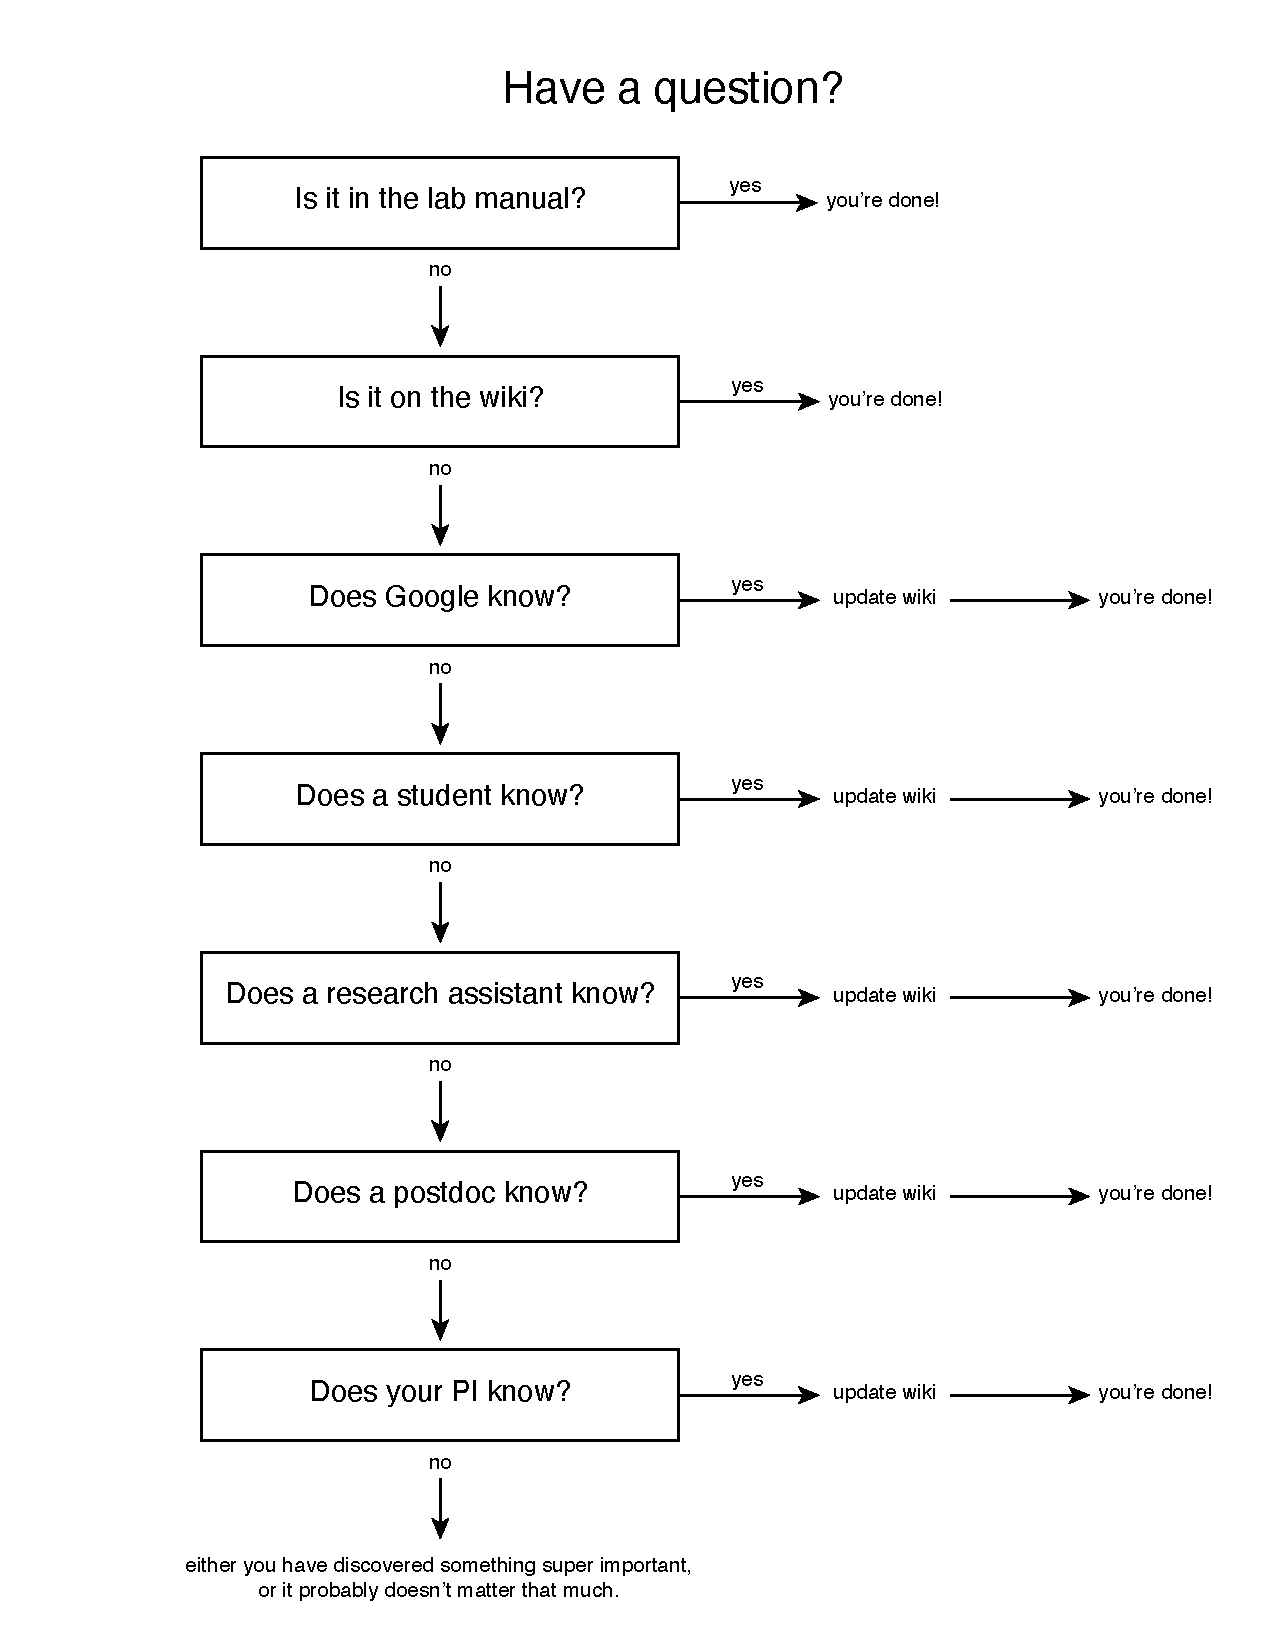
\includegraphics[width=\textwidth]{figures/lab_decision_tree.pdf}
\caption{A simple decision tree for questions and troubleshooting.}
\label{fig:decisiontree}
\end{figure}

\subsection{My Door}
Sometimes my physical door is closed.
\begin{itemize}[noitemsep]
\item When we have a meeting scheduled, knock.
\item When we do not have a meeting scheduled, a closed door usually means I am trying to write or focus. When it is urgent, knock anyway. Otherwise, send a Slack message.
\end{itemize}

\subsection{Lab Meetings}
Regular lab meetings help us maintain momentum on current projects and plan future work. Meetings are typically 60--90 minutes. In most weeks, we have one or two presenters who set the agenda and share materials in advance (e.g., a journal club plus a project update, practice talk, proposal, tutorial, or group discussion topic). Regular attendance and participation is expected of everyone making a sustained intellectual contribution to a project (see \Sref{sec:authorship} on \pref{sec:authorship}).

Treat lab meeting like a class: be prepared, be present, and be engaged. Read shared materials ahead of time, and avoid working on unrelated tasks during the meeting. When you are scheduled to present and need to cancel or postpone, give the group at least 72 hours notice when possible.

\subsection{Small-Group Data Meetings}
We sometimes hold small-group meetings focused on data, analyses, code, figures, or technical troubleshooting. These meetings are optional unless you are directly involved in the topic. Group troubleshooting is often more efficient than 1:1 help because others can learn at the same time and documentation can be updated immediately.

\subsection{Individual Meetings}
Senior lab members (postdocs, post-baccs, graduate students) typically meet with me weekly or biweekly. Come prepared. Assume we may only have 30 minutes, and aim to leave with clear next steps.

I do not schedule standing 1:1 meetings with most undergraduates, but I am available for ad hoc meetings (see scheduling instructions on Slab). Undergraduates should plan to meet with me at least once per semester.

\subsection{Slab}
Slab is where procedures, templates, and project records live. When you learn a workflow, solve a problem, or refine a procedure, document it so the next person can do the work faster and with fewer errors.

\subsection{Slack}
Slack is our primary tool for lab communication and day-to-day coordination. Use channels and threads so information stays searchable and visible.

\begin{itemize}[noitemsep]
\item Prefer channels over DMs for project work.
\item Use threads for follow-ups and updates.
\item When you assign or accept a task, make the owner and target date clear (when relevant) and define what ``done'' looks like.
\item Close the loop: reply in the same thread when complete, with links to relevant materials.
\end{itemize}

\subsection{Email}
Use Slack for most internal communication. Use email for formal or external communication (HR, departmental administration, faculty outside the lab who prefer email), and for anything that needs a durable record outside of Slack.

Email is not ideal for urgent issues. If something is time-sensitive, message me on Slack. If something is truly urgent, text/call me and/or the lab manager. If you cannot reach either of us and there is an immediate safety concern, follow Temple’s emergency guidance and contact emergency services as appropriate.

In general, read lab-related email and respond (when a response is needed) within one business day. When you will be away from email for more than a few days, use an out-of-office message.

\subsection{Calendars}
Accurate calendars help us manage lab space and shared resources. Use the lab calendars as instructed on Slab (attendance/away time, room scheduling, scanner bookings when relevant). Maintain your own calendar as well. When you receive a calendar invite for a meeting, accept it so the event is on your calendar.

%%%%%%%%%%%%%%%%%%%%%
\section{Communication Outside the Lab}

How you communicate outside the lab reflects on you and on the lab. This applies to research participants, collaborators, and scientific colleagues. Preparation matters. The less experience you have, the more you should plan and rehearse.

\subsection{Phone}
\begin{itemize}[noitemsep]
\item Answer the lab phone professionally and identify the lab and your name (e.g., ``Smith Lab, this is [Name]. How may I help you?'').
\item Check voicemail daily so nothing important slips through.
\item Return calls within one business day when possible. Follow study-specific procedures on Slab (and see \Sref{sec:participants} on \pref{sec:participants}).
\end{itemize}

\subsection{Manuscripts}
Scientific papers are one of the main ways we communicate our work and demonstrate scholarship. We have an obligation to communicate clearly and accurately.

\subsubsection{General}
\label{sec:ms_general}
Before drafting a manuscript, be familiar with George Gopen's \href{https://cseweb.ucsd.edu/~swanson/papers/science-of-writing.pdf}{``Reader Expectations''}. These principles reduce ambiguity and make writing easier to follow.

Additional Smith Lab drafting guidelines:
\begin{itemize}[noitemsep]
\item Start with a paragraph-level outline for each section, including key citations and claims.
\item When this is one of your first papers, plan to walk me through your outline before drafting full text.
\item Prioritize flow and structure. The reader does not know what you know.
\item Circulate drafts to all authors before submission and give them time to comment.
\item Read page proofs carefully, including references. Errors are common.
\end{itemize}

\noindent For authorship expectations, see \Sref{sec:authorship} on \pref{sec:authorship}.

\subsubsection{Formatting}
When sending me a draft:
\begin{itemize}[noitemsep]
\item Include a working title (or a few options), page numbers, and the full author list from the start.
\item Include placeholders for all sections, even when some are initially empty.
\item Use heading styles (do not rely on ad hoc bolding).
\item While we are iterating internally, keep text single-spaced and embed figures/tables near where they are discussed.
\end{itemize}

Your writing should be free of obvious spelling and grammar errors. Ask for help when needed (labmates, classmates, or the writing center: \url{http://www.temple.edu/writingctr/}).

\begin{shaded}
\noindent When you are sharing files outside of version-controlled systems, name files so they are both human- and machine-readable (e.g., \texttt{Lastname\_project\_v01.docx}). Avoid vague names like \texttt{Draft.docx}.
\end{shaded}

\subsubsection{Figures}
When we are still deciding what a figure should show, rough drafts are fine. When we already know the target, send the most polished version you can.

Figures should typically be vector art (e.g., PDF/EPS) when possible. Generate plots in R/Matlab/Python (or similar), then refine layout in a vector editor (e.g., Adobe Illustrator or Inkscape). Convert formats only when required for submission.

\begin{shaded}
\noindent Avoid making final figures in Excel or PowerPoint. They are fine for quick exploration, but they are rarely the best tools for publication-quality figures.
\end{shaded}

\subsubsection{Corresponding Authorship}
To keep the policy consistent and to ensure continuity of access to data and materials, I am the corresponding author for research conducted in the lab.

\subsection{Conference Presentations}
Anyone submitting an abstract should clear it with me first and circulate it to all authors at least one week before the submission deadline.

\subsubsection{Talks}
Anyone giving a talk to a non-lab audience must give a practice talk to the lab at least one week before the real talk. When it is your first public talk on a lab project, plan for at least two practice talks and start early.

\subsubsection{Posters}
Circulate a poster draft to all authors at least one week before the printing deadline. Confirm poster size and orientation early. A QR code linking to a PDF (hosted in an appropriate lab-approved location) can be helpful.

\begin{shaded}
\noindent Plan ahead for conference presentations. Unprepared or unprofessional behavior at a conference will affect future conference support.
\end{shaded}

\section{Communication with Everyone}
When appropriate, our work should be shareable with other researchers and the public. Assume that methods, de-identified outputs, and analysis code may eventually be shared (see \Sref{sec:openscience} on \pref{sec:openscience}). When you are unsure what can be shared (and where), ask before posting anything.


%%%%%%%%%%%%%%%%%%%%%
\chapter{Science}

\section{Scientific Integrity}
You have a responsibility to the lab, Temple, our sponsors, and the broader scientific community to uphold the highest standards of accuracy and integrity. There is never an excuse for fabricating, falsifying, or misrepresenting data or research progress. When you have questions about research practices, or concerns about something you have seen, talk to me immediately.

Integrity also includes day-to-day accuracy. Unintentional errors from rushing, inattentiveness, or poor documentation can be extremely damaging. Mistakes will happen, but we must catch them early, correct them transparently, and prevent them from recurring. Double-check your work frequently, and expect that key datasets and workflows will be independently checked by others.

When collecting data, use simple checklists so that each step has a clear owner and nothing is missed. Analyze and QC data as soon as feasible after collection so that problems are detected early rather than months later.

\section{Open, Accurate, and Reproducible Science}
\label{sec:openscience}

\subsection{Reproducibility and openness}
Our default is to make our work reproducible and shareable: materials, code, and de-identified outputs should be organized so that another researcher could understand and reproduce what we did. This is not about checking an ``open science'' box. It is about making our work usable by reviewers, collaborators, and future trainees.

\begin{itemize}[noitemsep]
\item \textbf{Organize data and metadata carefully.} Neuroimaging data should follow \href{https://bids.neuroimaging.io/}{BIDS} whenever applicable.
\item \textbf{Use GitHub for code.} Repositories must include a \texttt{README.md} that explains what the repository contains and how to reproduce key results.
\item \textbf{Write maintainable code.} Code should be tested, readable, and appropriately commented. For general guidance, see \href{https://journals.plos.org/ploscompbiol/article?id=10.1371/journal.pcbi.1006561}{``10 Simple Rules'' (Lee et al.)}.
\item \textbf{Use permanent links when sharing.} Prefer permanent identifiers (ideally DOIs) via \href{https://zenodo.org/}{Zenodo}, \href{https://figshare.com/}{FigShare}, or OSF (\href{http://help.osf.io/m/sharing/l/524208-create-dois-and-arks}{DOIs/ARKs}).
\end{itemize}

Some materials cannot be shared publicly (protected health information, identifiable data, or materials restricted by IRB or data use agreements). Our standard is: \textit{as open as possible, as closed as necessary}. When you are unsure what can be shared, ask before posting.

\subsection{Data management and computing}
Participant data are irreplaceable. Protect them and keep workflows reproducible.

\begin{itemize}[noitemsep]
\item Testing laptops should not leave the lab except for approved testing. Sign out equipment as described on Slab.
\item Do not install extraneous software or store personal files on lab computers.
\item Participant data should never live only on a testing machine or a personal device. Move data promptly after sessions and store them in approved lab locations.
\item Push code changes to GitHub regularly. Never commit identifiable data; commit only code and de-identified materials/outputs as appropriate.
\item Store manuscripts and shared writing in approved lab locations so drafts are backed up and accessible to collaborators.
\end{itemize}

\subsection{Accurate science and preventing mistakes}
Accuracy requires anticipating problems and building systems that reduce error. We will make mistakes, but we must learn from them and avoid repeating them.

Inspired by Rouder (2019; \href{https://doi.org/10.1177/2515245918801915}{Minimizing Mistakes in Psychological Science}), we aim to maintain a running log of problems and near-misses in Slab so we can learn from them and prevent repeats. This only works if we revisit it regularly, so we will make time each term to review the log, discuss patterns, and update our procedures. I include this here both as a commitment and as a reminder to make it happen.

\begin{itemize}[noitemsep]
\item A lab computer malfunctioning
\item A data transfer or analysis step failing (e.g., download from XNAT, corrupted export)
\item A missing or outdated software dependency that breaks a workflow
\item A budgeting or payment issue that risks interrupting recruitment (near-misses count)
\end{itemize}

When something does not go as planned, raise it. Silence is how small errors become large ones.

\section{Authorship}
\label{sec:authorship}

Authorship reflects responsibility and sustained intellectual contribution. Many journals and professional organizations provide guidelines (e.g., \href{http://www.icmje.org/recommendations/browse/roles-and-responsibilities/defining-the-role-of-authors-and-contributors.html}{ICMJE}). In this lab, two requirements are central:

\begin{enumerate}[noitemsep]
\item Contribute meaningfully to the intellectual scientific content (e.g., design, interpretation, theoretical framing).
\item Contribute meaningfully to the writing (e.g., outlining, drafting, revising, or substantive edits).
\end{enumerate}

Data collection and analysis are essential, but they do not automatically justify authorship on their own. Posters are often more inclusive than papers, so authorship on a poster does not automatically imply authorship on the paper. Undergraduates and research staff can earn paper authorship, but it requires learning enough of the background to engage intellectually and contributing substantively to writing.

Because projects can evolve over long timelines, author order (and, in rare cases, inclusion) may change to reflect actual contributions. Raise authorship questions early; clarity now prevents conflict later.

\section{Participants}
\label{sec:participants}

Our research depends on the goodwill and generosity of research participants. We need participants to feel respected, safe, and confident that we are competent and professional. Model interactions on other professional settings (e.g., a doctor's office).

For all participants:
\begin{itemize}[noitemsep]
\item Dress professionally when interacting with participants. When in doubt, ask.
\item Answer the phone and return calls/emails promptly. Identify yourself and the lab (e.g., ``Hello, this is [name] calling from the Smith Lab at Temple University...'').
\item Give clear task instructions and confirm understanding. When payments depend on choices, ensure participants understand how incentives work.
\item Be prepared to answer questions. When you do not know the answer, tell the participant you will follow up, and then make sure that happens quickly.
\item Arrive early enough to set up equipment and paperwork before the participant arrives (typically at least 30 minutes for in-lab testing). For off-campus meetups, arrive at the agreed meeting point early.
\end{itemize}

For non-students, and especially older adults, default to a title (Dr./Ms./Mr.) and last name. When you are unsure how to pronounce a name, ask.

Use participant-centered language (Table \ref{table:terms}):

\begin{table}
\centering
\caption{Participant-centered language}
\begin{tabular}{ll}
\toprule
Instead of saying: & Say this:\\
\midrule
experiment& study, research study\\
subject& volunteer, participant\\
test & task, screening, or game \\
\bottomrule
\end{tabular}
\label{table:terms}
\end{table}

Refer to Slab for study-specific procedures on recruiting, scheduling, and testing participants.

\section{Subject Payment}
\label{sec:subject_payment}
Participant payments must be tracked carefully. Follow the lab procedure for checking out payment materials, paying participants, and documenting payments. Each participant must sign the required payment documentation at the time of payment. When something seems off (missing forms, unclear balances, mismatched logs), raise it immediately.

\section{Testing Locations}
\label{sec:testing_locations}
\begin{itemize}[noitemsep]
\item Many testing locations are shared. Be a good citizen: schedule properly, use only allotted time, and leave the room clean.
\item Do not leave Smith Lab equipment in shared rooms (laptops, stimulation devices, cables, etc.). Equipment lives in the lab.
\item Do not test participants in a shared room unless you have properly reserved/signed out the space per the posted procedure.
\end{itemize}


%%%%%%%%%%%%%%%%%%%%%
\chapter{Professional Development}

\section{Recommendation Letters}
Writing letters of recommendation is part of my job, and I am glad to write strong letters for lab members when I can speak to their work. Please give as much notice as possible (ideally at least one month). In your request, include the deadline, the official name of the organization/program, what you are applying for, and any relevant instructions. Also send a current CV and a short list of specific examples you would like me to highlight. Ask early when anything is unclear.

\section{Staying on Top of the Literature}
\label{sec:literature}
Anyone aiming to make a sustained intellectual contribution to a project (see \Sref{sec:authorship} on \pref{sec:authorship}) should spend regular time each week reading and thinking about the relevant literature. New papers appear constantly, so the goal is not to read everything. The goal is to develop strong filters, build a mental model of the field, and learn to synthesize evidence.

As you read (or skim), keep asking:
\begin{itemize}[noitemsep]
\item What makes this paper persuasive or unpersuasive? What evidence supports the claims?
\item How does it connect to our lab's work and to your project specifically?
\item Where does it agree or disagree with other work, and why?
\item What new questions does it raise?
\end{itemize}

To manage volume, use multiple feeds and a system for organizing what you find:
\begin{itemize}[noitemsep]
\item Schedule time for reading and synthesis, especially when entering a new topic area.
\item Use alerts (journal TOCs, PubCrawler, and Google Scholar alerts for topics or authors).
\item Use a reference manager (e.g., Zotero) to save PDFs, add notes, and organize themes.
\item Review what you saved and write short syntheses that connect papers (even a few paragraphs per month adds up).
\item Share useful papers and ideas with the lab (in \texttt{papers-*} Slack channels and during lab meetings).
\end{itemize}

\begin{shaded}
\noindent The goal is simple: read widely enough to recognize patterns, and synthesize clearly enough to explain how the pieces fit together.
\end{shaded}

\section{Learning to Code}
\label{sec:coding}

Coding is an essential skill in modern psychology and neuroscience\footnote{\url{http://www.russpoldrack.org/2016/05/advice-for-learning-to-code-from-scratch.html}}. Comfort with programming (especially Python and Matlab, and often R) enables you to build tasks, manage data, run analyses, and create reproducible workflows.

Most people learn coding through a mix of online materials, documentation, mentorship, and practice. Learning goes fastest when you have a concrete goal (e.g., analyze a dataset, build a task, automate QC).

\subsection{Using AI tools (LLMs) well}
AI coding assistants (including large language models) can be useful for learning, debugging, and accelerating routine work. I encourage you to use them---with two constraints: they should not replace your understanding, and you are still responsible for correctness, transparency, and reproducibility.

A helpful recent set of principles is summarized in the preprint \textit{Ten Simple Rules for AI-Assisted Coding in Science}\footnote{\href{https://arxiv.org/abs/2510.22254}{https://arxiv.org/abs/2510.22254}}. In practice:

\begin{itemize}[noitemsep]
\item Use AI as a tutor or pair programmer: ask for explanations, small examples, and alternatives---not just a finished answer.
\item Be explicit about inputs, outputs, constraints, and edge cases. The quality of the result depends on the quality of the specification.
\item Treat generated code as a first draft. Read it, simplify it, and make sure you could explain it to someone else.
\item Validate aggressively: write tests when possible, run sanity checks, and confirm that results reproduce from a clean environment.
\item Keep changes small and version-controlled so mistakes are easy to find and undo.
\item Never paste participant-identifying information, protected data, or anything confidential into an AI tool.
\end{itemize}

\subsection{While learning, keep these principles in mind}
\begin{itemize}[noitemsep]
\item Be patient and persistent. Everyone gets stuck; progress comes from repeated attempts.
\item Be careful and systematic. Many failures come from small typos or path mistakes.
\item Understand inputs and outputs for scripts you run. Avoid treating code as magic.
\item Learn directory structure and paths. Many errors are file-location errors.
\item If you have stared at the same problem for 30 minutes without progress, switch tasks, take a short break, or ask for help.
\item Ask for help early and clearly. Labmates and forums (e.g., NeuroStars) are good resources. You can also post to the lab troubleshooting channel on Slack.
\end{itemize}

\begin{shaded}
\noindent Learning to code can be frustrating, but the payoff is large. These skills generalize to virtually every research setting and to many industry roles.
\end{shaded}

\section{Effective Menteeship}
Mentoring is a core part of how our lab works. As you gain experience, you should expect to teach and support others who are more junior. At the same time, everyone remains a mentee, and effective menteeship is a skill.

A practical starting point is the ``golden rules'' framework described by \href{https://doi.org/10.1136/bmj.i4147}{Chopra et al.\ (2016)} and related discussions of ``managing up'' (e.g., \href{https://doi.org/10.1097/ACM.0b013e3181906e8f}{Zerzan et al.\ 2009}). In practice, effective menteeship usually means:

\begin{itemize}[noitemsep]
\item Respect your mentor's time by coming prepared and keeping requests specific.
\item Communicate clearly: summarize context, state the question, and propose next steps.
\item Take ownership over the relationship: track action items, follow through, and raise issues early.
\item Stay engaged and collaborative, especially when work is difficult or ambiguous.
\end{itemize}

\end{document}
